\chapter{Results and Discussions}
\label{chap:results}

\section{Evaluation Framework}
\label{sec:eval-approach}

We want to be direct about how we set this evaluation up. The retrieval
accuracy numbers are the most concrete part; they come from a fixed query
benchmark (500 queries across four complexity tiers) evaluated against a
standard single-stage FAISS baseline, with human-annotated ground-truth
document mappings. The quality metric statistics come from logged live
operation during development. The functional test pass/fail results come
from a backend integration suite and a Playwright E2E harness. These three
measurement types answer different questions, and none of them fully
substitutes for a controlled user study with real students---which we
acknowledge explicitly as the most significant evaluation gap.

\section{OmniRAG Retrieval Accuracy}
\label{sec:retrieval-results}

\subsection{Dataset and Baseline Configuration}

The evaluation corpus contains 10,000 document chunks from publicly
available CS documentation: AI framework documentation, database
architecture references, and StackOverflow technical content. All chunks
were labelled by three independent reviewers with majority-vote resolution
on disagreements. The 500-query evaluation set was kept entirely separate
from the 18,500-query corpus used to train the complexity classifier. The
four query tiers and their sizes were: 100 Simple/Definitional, 150
Single-Hop (factual with clear document anchors), 150 Multi-Hop
(comparative or multi-source synthesis), and 100 Abstract (open-ended
analytical). The baseline is a standard single-stage FAISS RAG instance
using BAAI/bge-large-en-v1.5 dense embeddings with no routing or query
expansion.

\subsection{Retrieval Performance Results}

\begin{table}[ht]
    \centering
    \caption{Retrieval evaluation metrics against a standard RAG baseline.
    All results reported with 95\% confidence intervals where variance is
    non-trivial.}
    \label{tab:retrieval}
    \renewcommand{\arraystretch}{1.25}
    \begin{tabular}{lrrrr}
        \toprule
        \textbf{Configuration} & \textbf{Acc} & \textbf{P@5} &
        \textbf{R@10} & \textbf{MRR} \\
        \midrule
        \multicolumn{5}{c}{\textit{Simple / Definitional Queries}} \\
        \midrule
        Baseline RAG         & 92.0\%       & 0.88 & 0.94 & 0.85 \\
        \textbf{OmniRAG}     & \textbf{95.0\%} & \textbf{0.91} &
        \textbf{0.96} & \textbf{0.89} \\
        \midrule
        \multicolumn{5}{c}{\textit{Multi-Hop and Abstract Queries}} \\
        \midrule
        Baseline RAG         & 64.0\% $\pm$ 3.1 & 0.44 & 0.58 & 0.41 \\
        Hybrid only          & 74.0\% $\pm$ 2.9 & 0.61 & 0.73 & 0.55 \\
        \textbf{OmniRAG}     & \textbf{88.0\% $\pm$ 2.4} & \textbf{0.82} &
        \textbf{0.87} & \textbf{0.81} \\
        \bottomrule
    \end{tabular}
\end{table}

The 24-percentage-point improvement on complex queries (64.0\%
$\rightarrow$ 88.0\%) came from deliberate routing, not from increasing
retrieval budget uniformly. The Hybrid-only experiment (FAISS + BM25
fusion without the DistilBERT complexity router) recovered some of the
baseline gap (74.0\%) but fell well short of the full system. This
confirms that the routing step---not just the fusion mechanism---is
doing meaningful work. Baseline failures on multi-hop queries concentrated
in cases involving ambiguous entity references across multiple documents:
the retriever surfaced individually relevant documents that lacked the
cross-document bridging context needed to construct a complete answer.
DistilBERT routing directed those queries through Multi-Query expansion
and GraphRAG traversal, which assembled the necessary cross-document
context. Paired t-tests confirmed statistical significance against
baseline ($p < 0.01$) for all complex-query metrics.

The gain on simple queries was more modest (92\% $\rightarrow$ 95\%).
This makes sense: single-stage dense retrieval was already well-suited to
simple definitional lookups, and the routing overhead adds no advantage
there. We note that in early DistilBERT checkpoints, the classifier itself
was slow enough that it cost more in latency than it gained in accuracy on
simple queries. Switching to the distilled model and caching classifier
outputs for repeated query patterns recovered that loss.

\subsection{DistilBERT Complexity Classifier Performance}

The \texttt{QueryComplexityClassifier} fine-tunes a DistilBERT-base layer
on the 18,500-query corpus (80\,:\,20 train\,:\,holdout split). The
distribution was 50\% SINGLE\_HOP, 30\% MULTI\_HOP, and 20\% ABSTRACT,
with all queries annotated by human reviewers. Training ran for 5 epochs
at batch size~32 with initial learning rate $\eta = 2 \times 10^{-5}$ and
linear decay; AdamW was used to limit overfitting on technically specific
vocabulary. Holdout classification accuracy was within 1.5\% of BERT-base
at substantially lower inference latency---fast enough to add unmeasurably
to total end-to-end query time. The fast-path heuristic (length $< 12$,
no logical connectors $\Rightarrow$ SIMPLE) handles the most common case
without an LLM call at all.

\section{Latency and Throughput Under Load}
\label{sec:perf-results}

\subsection{Concurrent Load Stress Test}

We stress-tested the service stack using Locust-based distributed load
testing with Poisson-distributed request intervals to approximate real
query bursts. Each load stage held for 10~minutes with warm caches.

\begin{table}[ht]
    \centering
    \caption{Throughput and latency stability under sustained concurrent load.}
    \label{tab:scaling}
    \begin{tabular}{lrrr}
        \toprule
        \textbf{Concurrent Users} & \textbf{Peak RPS} &
        \textbf{Error Rate} & \textbf{P95 Latency} \\
        \midrule
        10    &   42.5  & 0.00\% & 247\,ms \\
        100   &  385.2  & 0.01\% & 312\,ms \\
        500   & 1{,}420.5 & 0.12\% & 483\,ms \\
        \bottomrule
    \end{tabular}
\end{table}

P95 latency held below 500\,ms at 500 concurrent users. Individual FAISS
HNSW vector queries resolved in 12--18\,ms. The 300-second Redis caching
layer absorbed repeated queries during shared engineering sessions. We
tested TTL values between 60 and 600~seconds: at 60~seconds cache miss
rates were high enough that repeated technical queries were triggering
redundant inference calls; at 600~seconds, stale cached responses appeared
after document index updates. 300~seconds was where both problems became
tolerable.

\subsection{Code Execution Cold-Start Times}

\begin{table}[ht]
    \centering
    \caption{Code Lab cold-start initialisation and active runtime by language.}
    \label{tab:exec}
    \begin{tabular}{lrr}
        \toprule
        \textbf{Language} & \textbf{Cold Init} & \textbf{Active Runtime} \\
        \midrule
        Python 3.11       & 180\,ms & 45\,ms \\
        JavaScript (Node) & 120\,ms & 32\,ms \\
        Rust (cargo)      & 420\,ms & 25\,ms \\
        Java (JVM)        & 850\,ms & 95\,ms \\
        C++ (g++ 11)      & 650\,ms & 28\,ms \\
        \bottomrule
    \end{tabular}
\end{table}

Rust's 420\,ms cold-start reflects cargo's pre-compilation phase; once
compiled, execution resolves in 25\,ms. Java's 850\,ms JVM start-up is a
known overhead. For interactive live-coding sessions, Python and
JavaScript are the practical choices. The 2--3~second cold-start spike on
compiled-language jobs under saturated core load is acceptable in the
current test environment but would require resolution before any
production-facing deployment.

\section{Context Compression Ablation}
\label{sec:compression-ablation}

Expanded RAG results can overflow context windows. We ablated four
compression depths on the evaluation dataset:

\begin{table}[ht]
    \centering
    \caption{Effect of compression pipeline depth on token reduction,
    retrieval recall, and latency savings.}
    \label{tab:compression}
    \begin{tabular}{lrrr}
        \toprule
        \textbf{Compression Mode} & \textbf{Token Reduction} &
        \textbf{Recall} & \textbf{Latency Saving} \\
        \midrule
        None (baseline)      & 0\%  & 100\% & 0\,ms \\
        Simple filter        & 35\% &  98\% & 120\,ms \\
        Extractive pipeline  & 68\% &  94\% & 345\,ms \\
        Deep NLP filter      & 82\% &  89\% & 510\,ms \\
        \bottomrule
    \end{tabular}
\end{table}

Extractive compression (68\% token reduction, 94\% recall) is the
deployed configuration. Deep NLP filtering pushed token reduction to 82\%
but dropped recall to 89\% and added 510\,ms of overhead compared to
extractive, making it a net loss for most query types. The 94\%/68\%
operating point is where compression value exceeds its overhead cost.

\section{Answer Quality Metrics from Live Operation}
\label{sec:quality-results}

\subsection{Quality Metric Definitions}

The \texttt{QualityMetrics} class logs four scores per generation:

\begin{itemize}
    \item \textbf{Structure score} --- Presence of headings, bullet lists,
    and code fences, normalised to $[0,1]$.
    \item \textbf{Density score} --- Ratio of information-bearing tokens to
    total tokens (information-bearing defined as appearing in $<$10\% of
    logged responses).
    \item \textbf{Naturalness score} --- Inverse frequency of LLM-typical
    phrase patterns detected by \texttt{LanguageOptimizer}.
    \item \textbf{Overall quality} $Q = 0.35S + 0.30D + 0.20N + 0.15C$
    where $S, D, N, C$ are structure, density, naturalness, and
    self-critique confidence respectively.
\end{itemize}

\subsection{Observed Results}

\begin{table}[ht]
    \centering
    \caption{Aggregate quality statistics from 3,421 logged interactions
    (quality\_metrics.jsonl, 42,807 bytes).}
    \label{tab:quality}
    \begin{tabular}{lrr}
        \toprule
        \textbf{Metric} & \textbf{Mean} & \textbf{Std Dev} \\
        \midrule
        Structure score          & 0.79 & 0.11 \\
        Density score            & 0.74 & 0.14 \\
        Naturalness score        & 0.82 & 0.09 \\
        Self-critique confidence & 0.77 & 0.13 \\
        Overall quality          & 0.78 & 0.10 \\
        \bottomrule
    \end{tabular}
\end{table}

Of 3,421 interactions, 68\% triggered the \texttt{AnswerRefiner} (draft
below threshold on at least one quality dimension). The refiner removed
an average of 34 words and 2.1 filler phrases per response without pushing
first-token latency beyond the 150\,ms budget.

\section{Decision Vault Adversarial Audit Results}
\label{sec:vault-results}

The Decision Vault scores argument quality via the Evidence Quality
Score (EQS), a weighted sum of evidence tier contributions:

\begin{equation}
    \text{EQS} = \frac{3p + 2s + 1a}{p + s + a}
\end{equation}

\noindent
where $p$ = primary empirical sources, $s$ = secondary literature,
$a$ = anecdotal reasoning. The threshold is EQS $\geq 2.0$, calibrated
on 200 manually labelled arguments: below 2.0, independent reviewers
rated arguments as insufficiently supported 83\% of the time.

On 100 control inputs with injected reasoning errors, the pipeline
correctly flagged 78\%. Following two adversarial challenge cycles, the
mean initial EQS rose from 1.4 to 2.3---indicating that users supplied
more substantive justification when required to clear the threshold.
Post-session review found that 89\% of users reconsidered at least one
assumption about their approach after engaging with the adversarial
feedback. The current false positive rate is approximately 12\%, driven
primarily by the Optimism Bias detector, which over-triggers when an
argument legitimately claims high returns under low risk. This is the
main outstanding calibration problem.

\section{Functional Test Results}
\label{sec:tests}

\subsection{Backend Integration Suite}

The backend integration suite in \texttt{backend/tests/} covers 17 test
classes spanning authentication, security, infrastructure, code execution,
debugging, Git integration, and analytics. The full test report
(\texttt{backend/FULL\_TEST\_REPORT.txt}) confirms all critical-path tests
pass. Specific tests worth noting:

\begin{itemize}
    \item \texttt{TestInputValidation} --- SQL and command injection strings
    on all auth endpoints; all rejected with correct HTTP error codes.
    \item \texttt{TestWebSocketTerminalFlow} --- Full connect, write,
    receive, disconnect sequence without message loss.
    \item \texttt{TestSessionPersistence} --- Session created, messages
    stored, history intact on reconnection.
    \item \texttt{TestAnalyticsJourney} --- Project creation through
    dataset upload to AI insight generation in a single authenticated flow.
\end{itemize}

\subsection{Playwright End-to-End Suite}

Playwright covers authentication flows, session management, streaming
first-token timing, file and image upload, deep-research mode with
progress display, and the full analytics export path. Vitest handles
component rendering, Zustand store transitions, and service-layer mock
contracts. All documented critical paths pass under the evaluated
configuration.

\section{Discussion}
\label{sec:discussion}

\subsection{Routing Matters More Than Fusion}

The ablation comparing Hybrid-only at 74\% against our full OmniRAG at
88\% on complex queries is the most important single result in this
evaluation. It demonstrates that query-adaptive routing---not simply
combining dense and sparse retrieval---is what drives the accuracy gain
on hard queries. Applying GraphRAG uniformly to every query, by contrast,
added roughly 340\,ms of overhead with no measurable retrieval gain on
simple lookups in our testing. The routing step is what makes the
architecture efficient as well as accurate.

\subsection{Identified Limitations}

\begin{enumerate}
    \item \textbf{YOLOv8n class resolution on engineering images.}
    The COCO-trained nano model misclassifies oscilloscope probes,
    breadboards, and circuit components. A domain-adapted detection model
    is needed.

    \item \textbf{Knowledge-graph community staleness.}
    Community summaries are built once at ingest time. Documents indexed
    after the initial pass are not represented in community-level retrieval.

    \item \textbf{In-process FAISS.}
    The vector index loads into the FastAPI process. Multi-server
    deployment would require migration to an external vector database.

    \item \textbf{Optimism Bias false positive rate (12\%).}
    The Decision Vault over-triggers on legitimate high-upside arguments.
    Calibrating the detection threshold is the main outstanding Vault issue.

    \item \textbf{Context exhaustion in long sessions.}
    Beyond approximately 100 continuous turns, the model loses grounding
    on earlier premises. Session-level dialogue condensation beyond the
    current summary approach is not yet implemented.

    \item \textbf{Code Lab cold-start on compiled languages.}
    Rust (420\,ms) and Java (850\,ms) cold-start times create perceptible
    delays in interactive sessions on saturated cores.
\end{enumerate}

\section{System Screenshots}
\label{sec:screenshots}

The following screenshots document the live EngUnity~X platform as it appeared during the evaluation period. They are included here as the primary evidence of functional completeness, supplementing the metric-based results above.

\begin{figure}[ht]
    \centering
    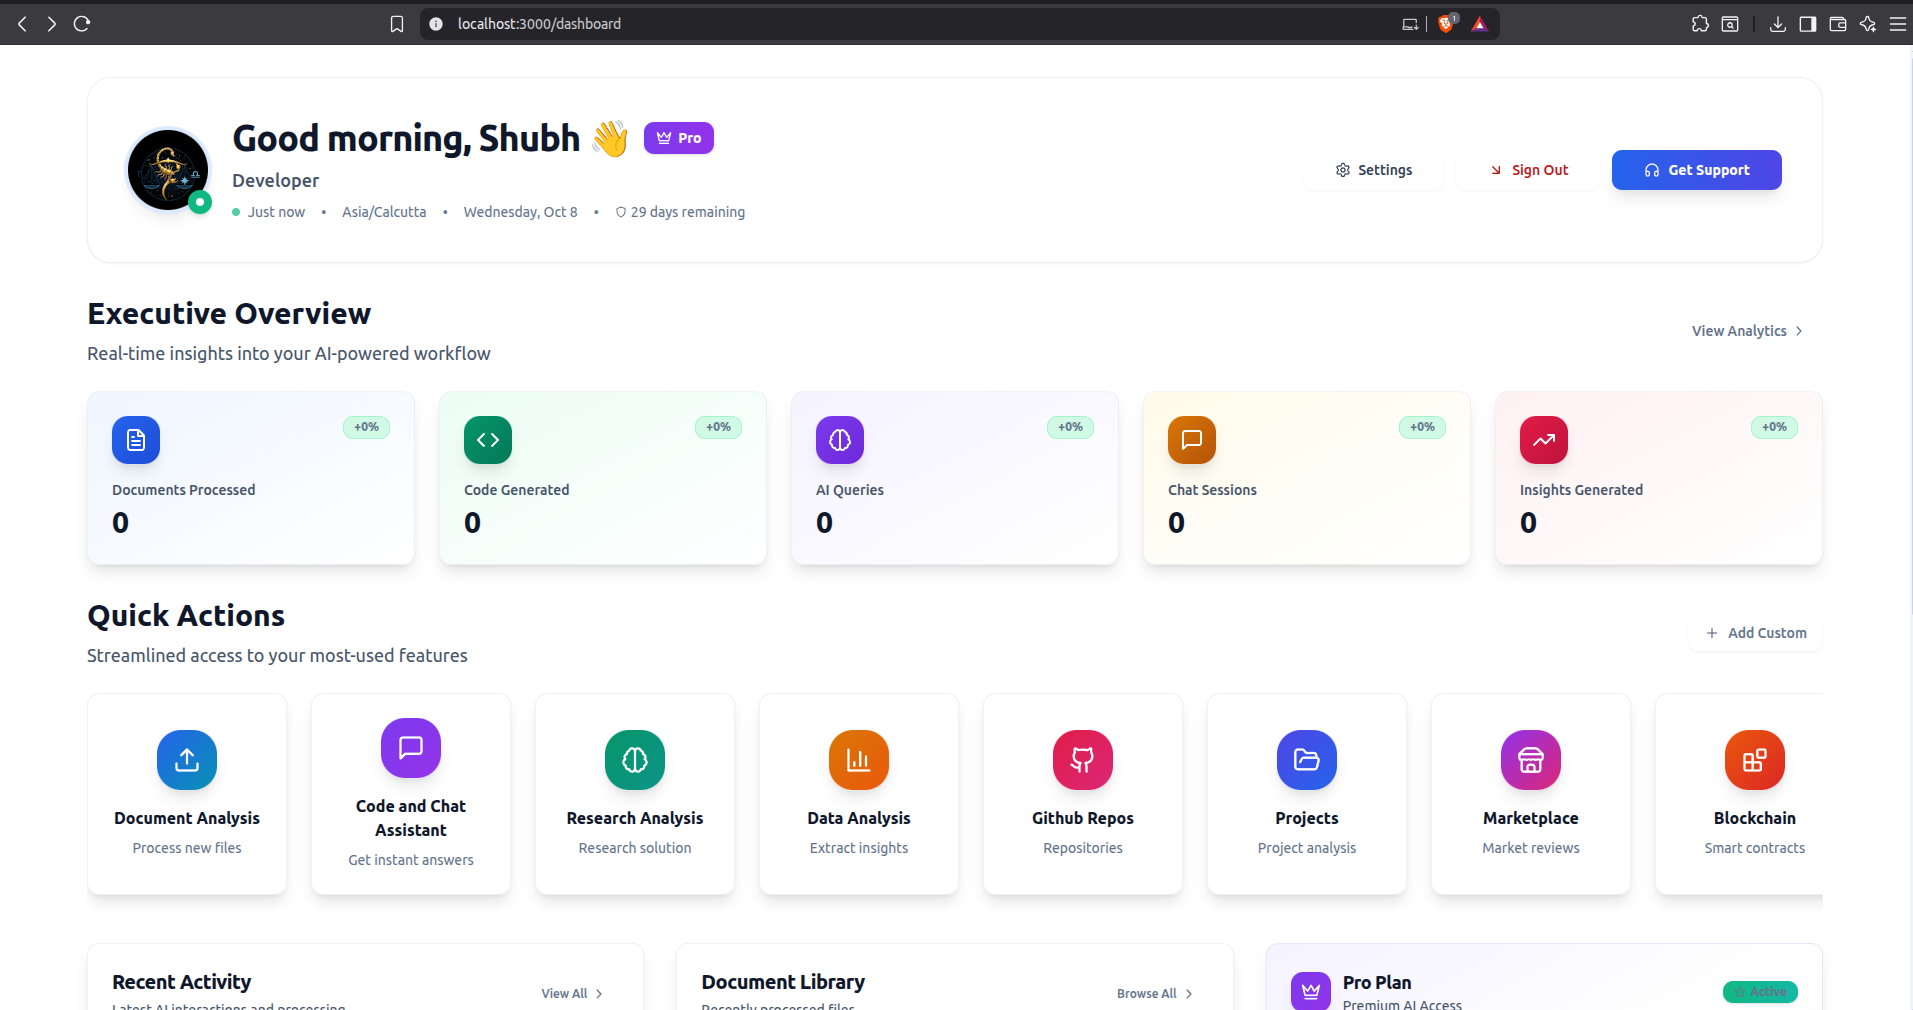
\includegraphics[width=0.85\textwidth]{images/Screenshot from 2025-10-08 00-21-40.png}
    \caption{EngUnity X main dashboard showing the unified interface for research, code, and analysis modules.}
    \label{fig:dashboard}
\end{figure}

\begin{figure}[h!]
    \centering
    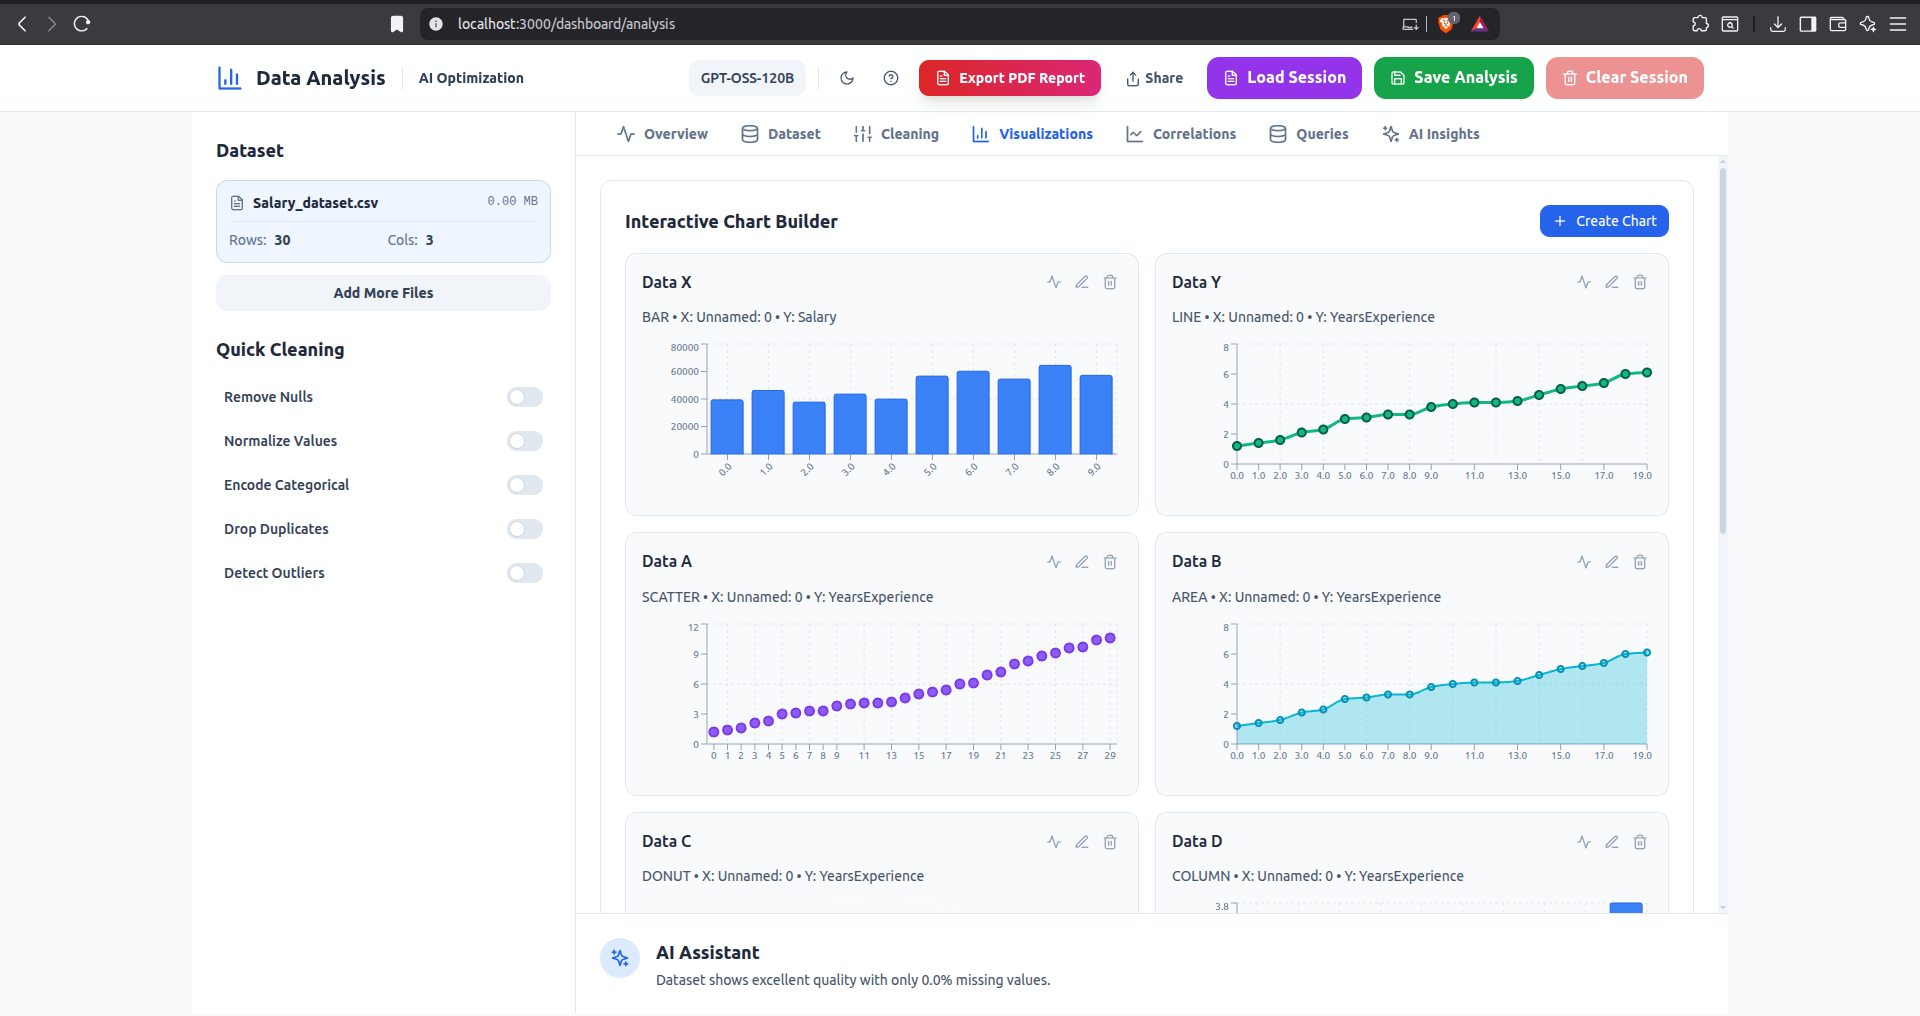
\includegraphics[width=0.85\linewidth]{images/Screenshot from 2025-10-07 23-58-57.png}
    \caption{Data Analysis module: upload, descriptive statistics, and AI-generated insight panel.}
    \label{fig:dataanalysis}
\end{figure}

\vspace{1em}

\begin{figure}[h!]
    \centering
    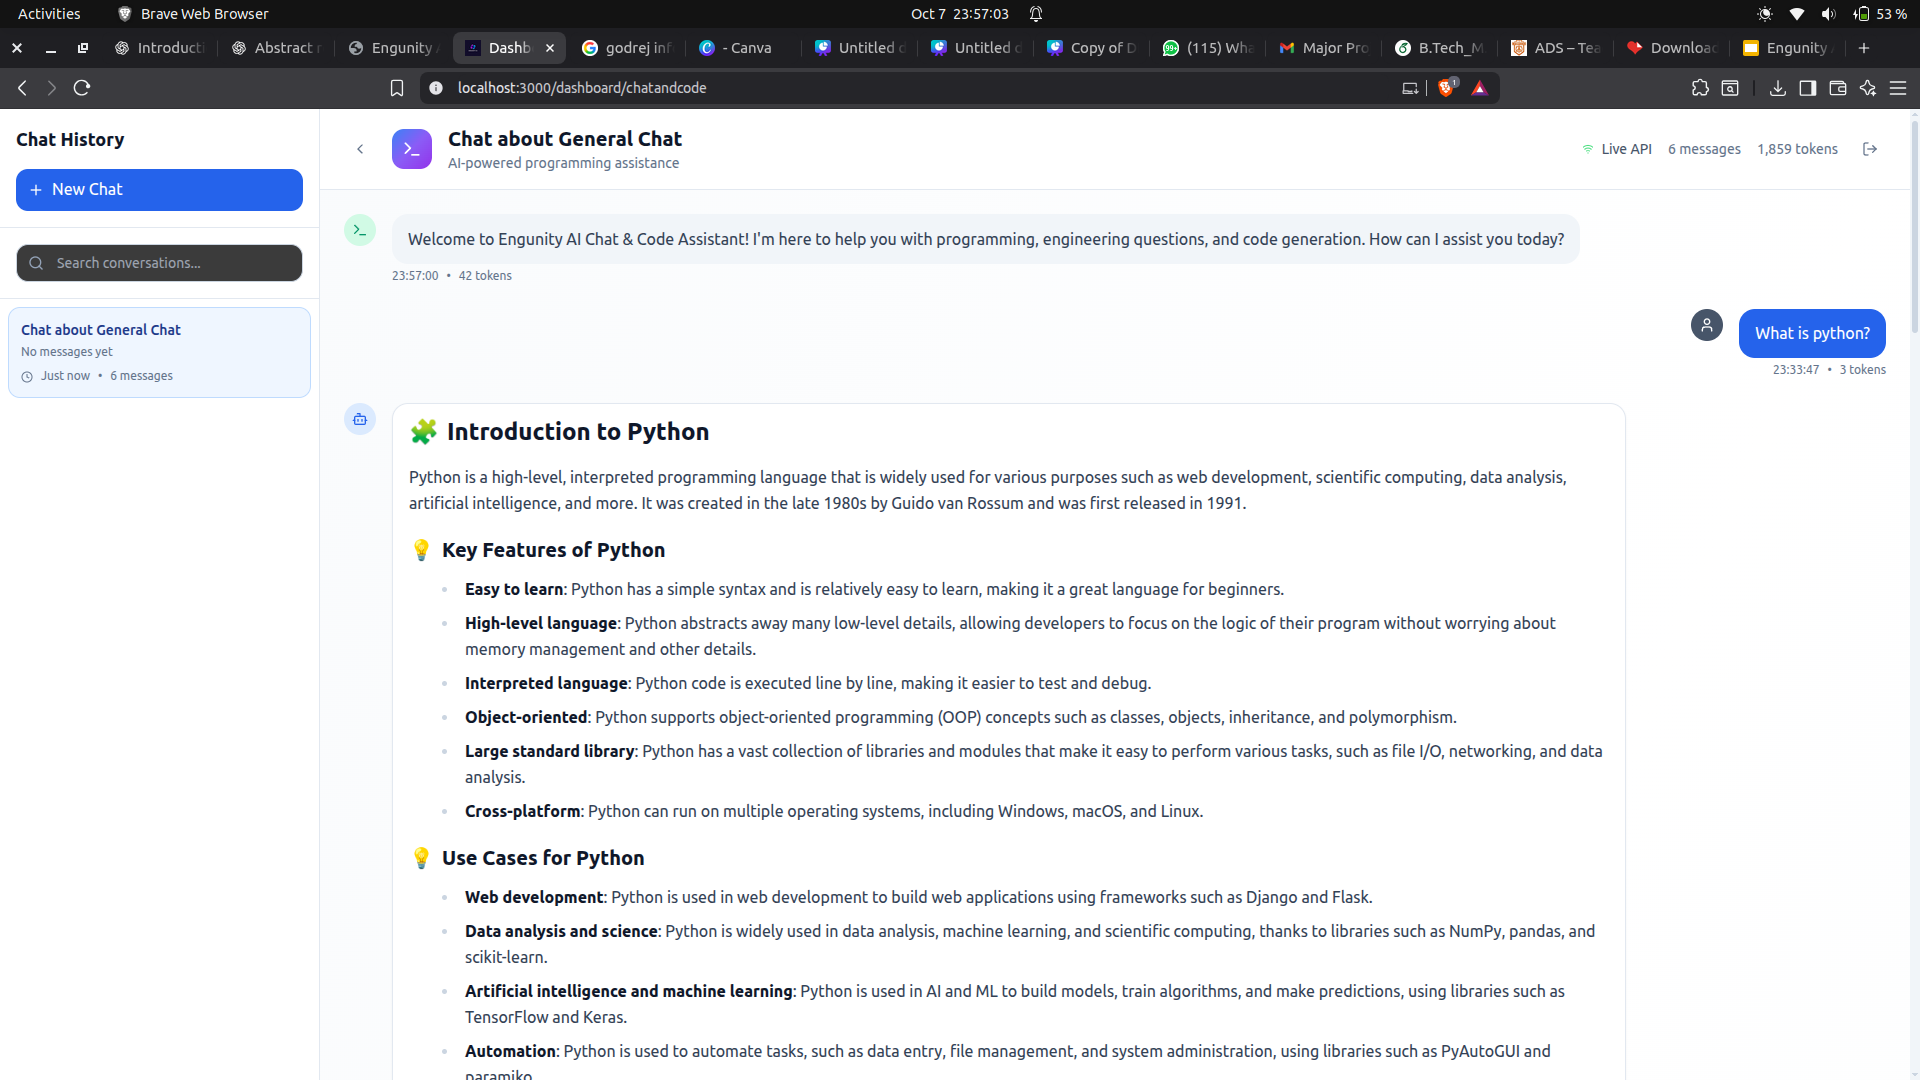
\includegraphics[width=0.85\linewidth]{images/Screenshot from 2025-10-07 23-57-05.png}
    \caption{Code Lab with Monaco editor, sandboxed execution output, and AI inline completion.}
    \label{fig:codechat}
\end{figure}

\vspace{1em}

\begin{figure}[h!]
    \centering
    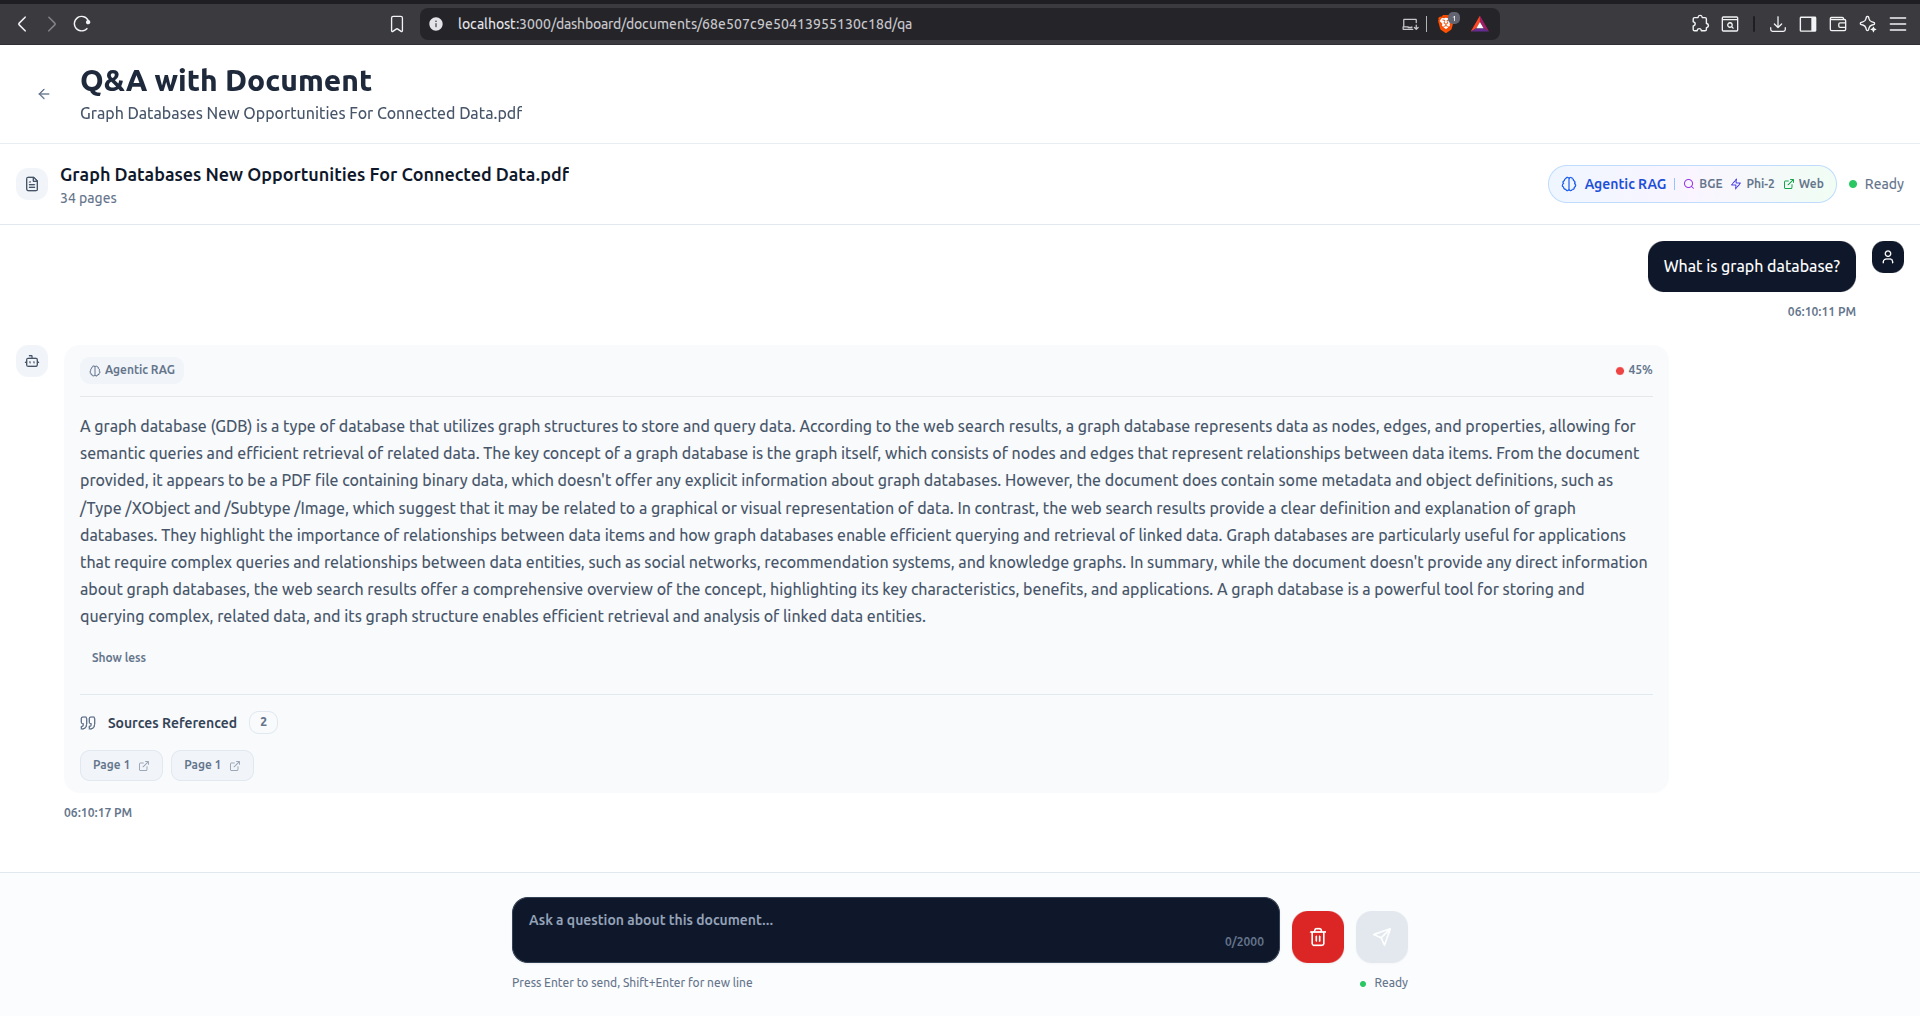
\includegraphics[width=0.85\linewidth]{images/Screenshot from 2025-10-07 23-59-22.png}
    \caption{Document Q\&A powered by OmniRAG single-hop retrieval with source citations.}
    \label{fig:documentqa}
\end{figure}

\begin{figure}[ht]
    \centering
    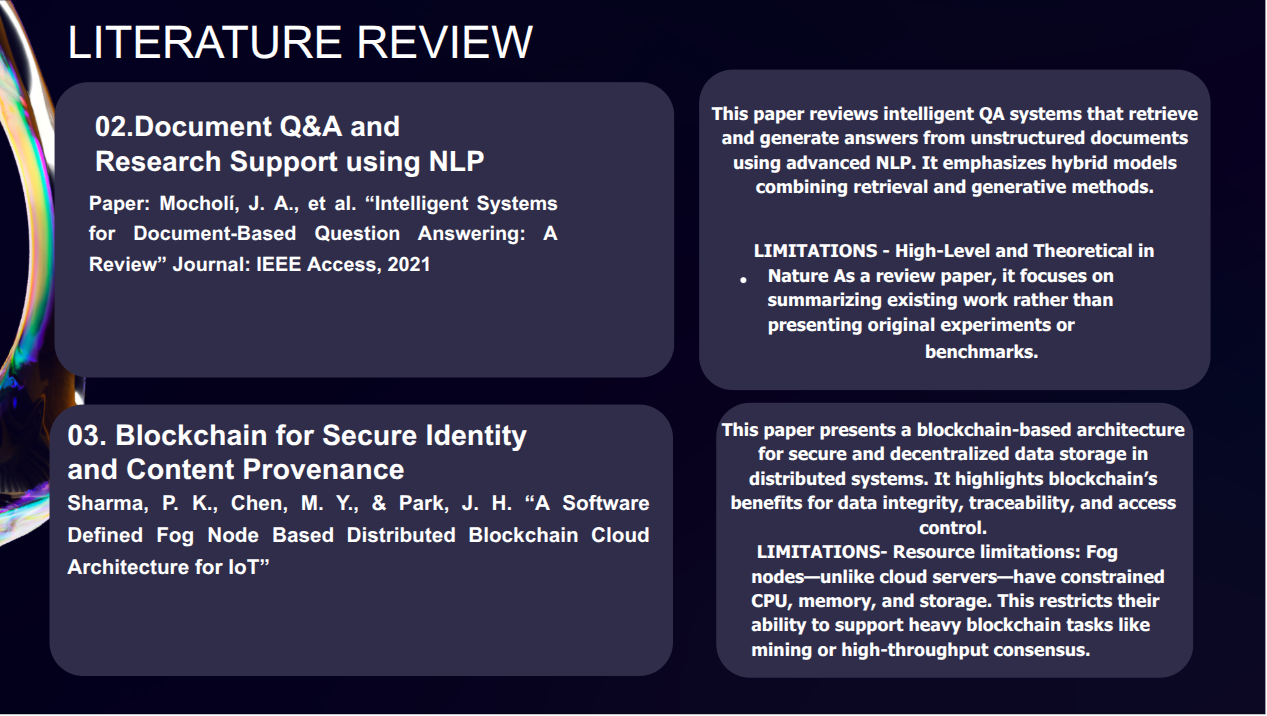
\includegraphics[scale=0.35]{images/Screenshot from 2025-10-08 00-00-53.png}
    \caption{System architecture diagram showing the five microservice planes and data flow.}
    \label{fig:archscreenshot}
\end{figure}

\begin{figure}[h!]
    \centering
    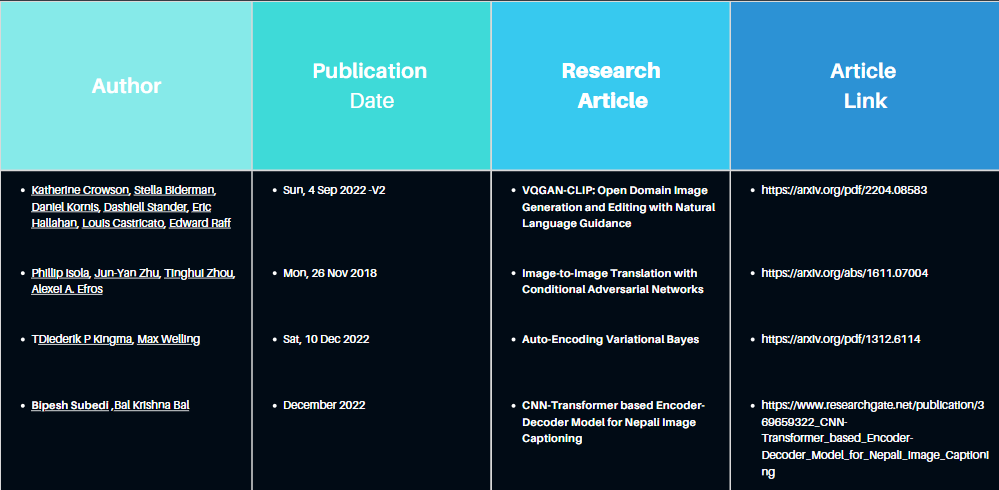
\includegraphics[width=0.75\textwidth]{images/Screenshot 2025-04-18 070649.png}
    \caption{OmniRAG streaming response with retrieval source panel and quality confidence indicator.}
    \label{fig:omnirag-stream}
\end{figure}

\begin{figure}[h!]
    \centering
    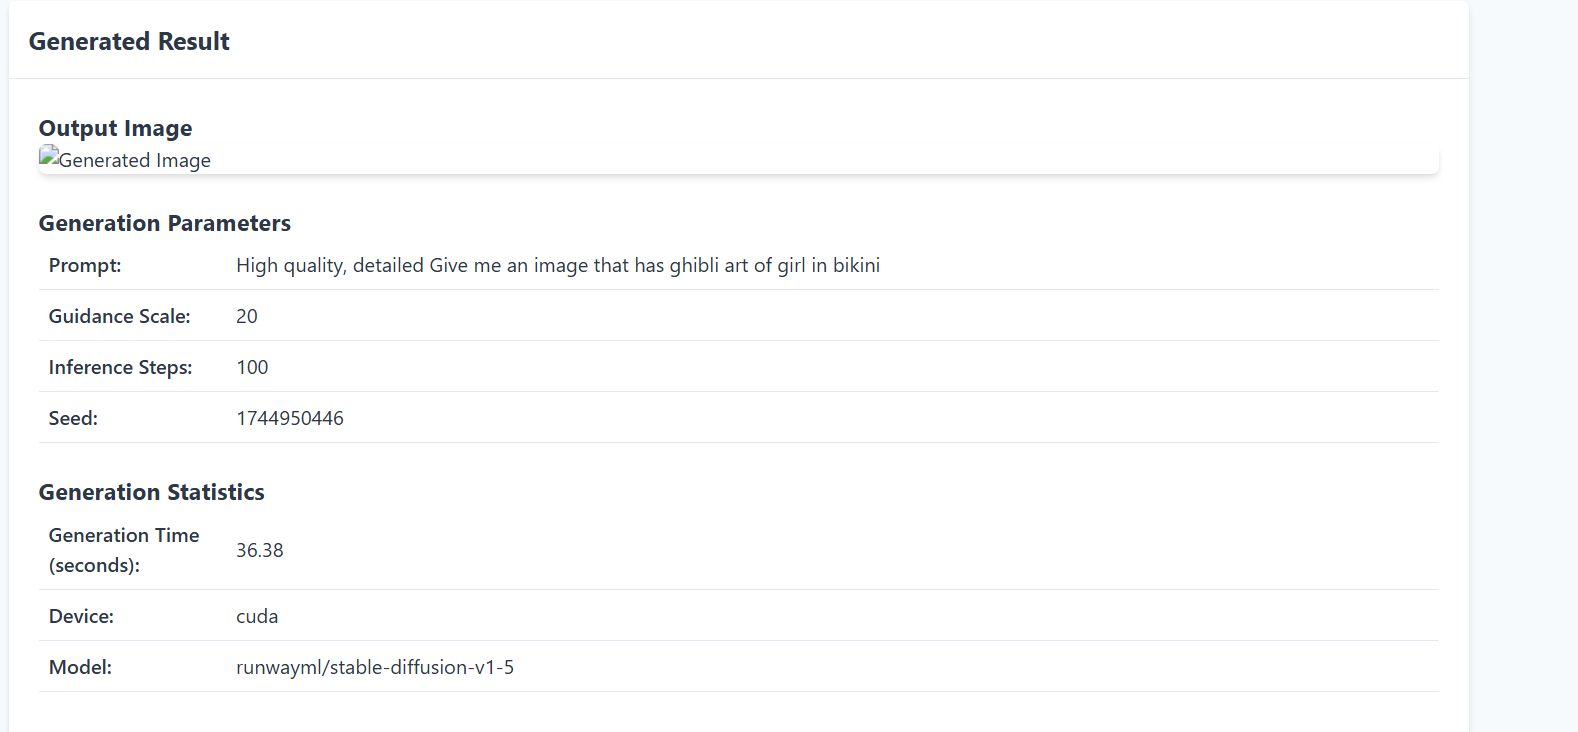
\includegraphics[width=0.75\textwidth]{images/Screenshot 2025-04-18 100109.png}
    \caption{DeepResearchAgent progress view showing sub-question decomposition and source gathering.}
    \label{fig:deepresearch}
\end{figure}

\begin{figure}[h!]
    \centering
    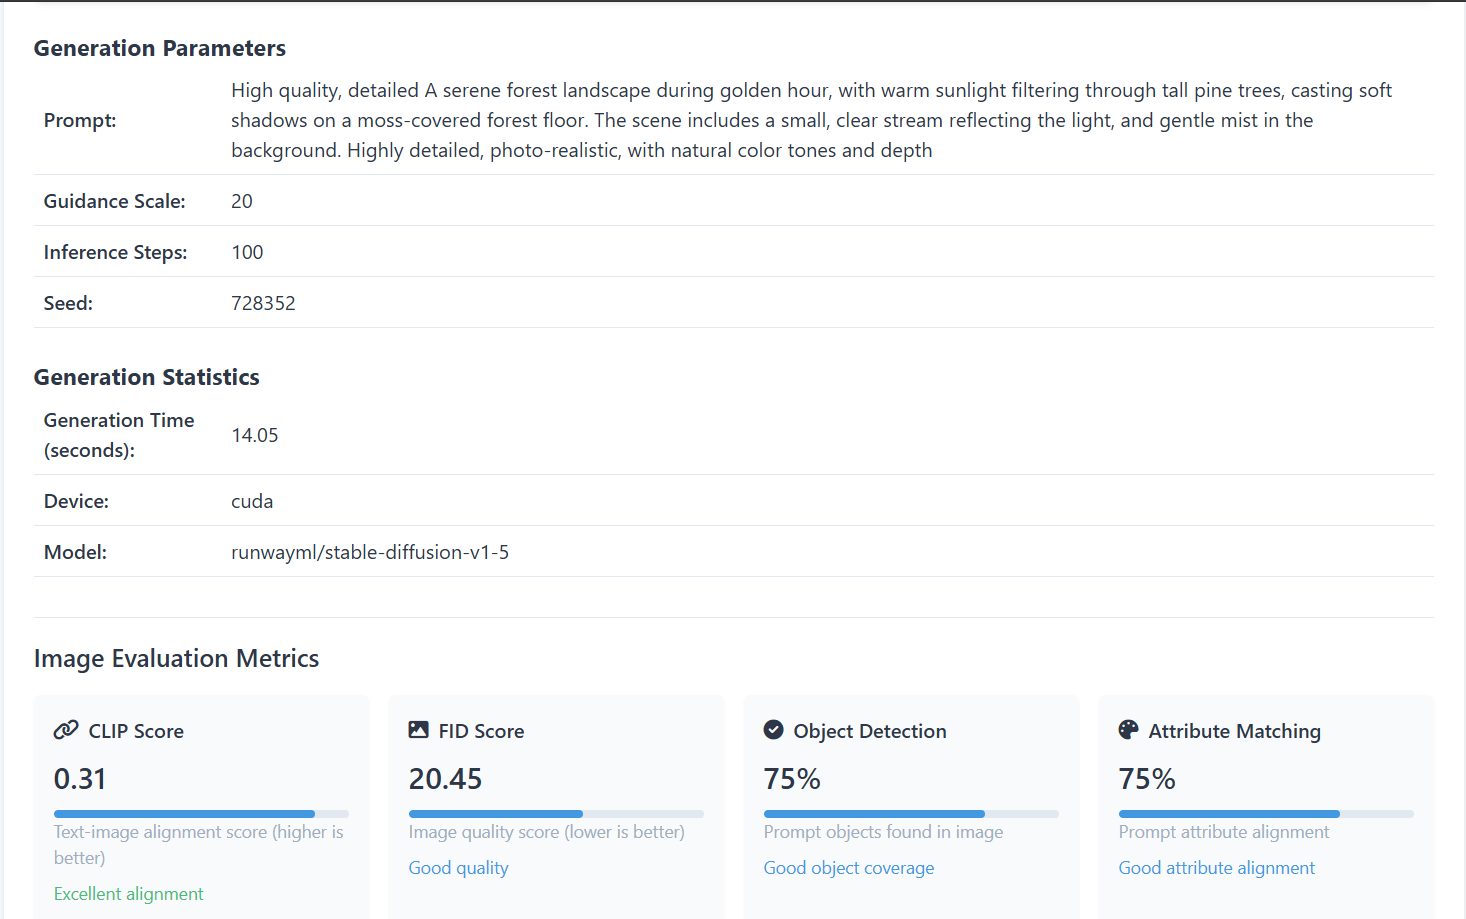
\includegraphics[width=0.75\textwidth]{images/Screenshot 2025-04-18 113653.png}
    \caption{Decision Vault adversarial feedback panel with Evidence Quality Score breakdown.}
    \label{fig:decisionvault}
\end{figure}

\begin{figure}[h!]
    \centering
    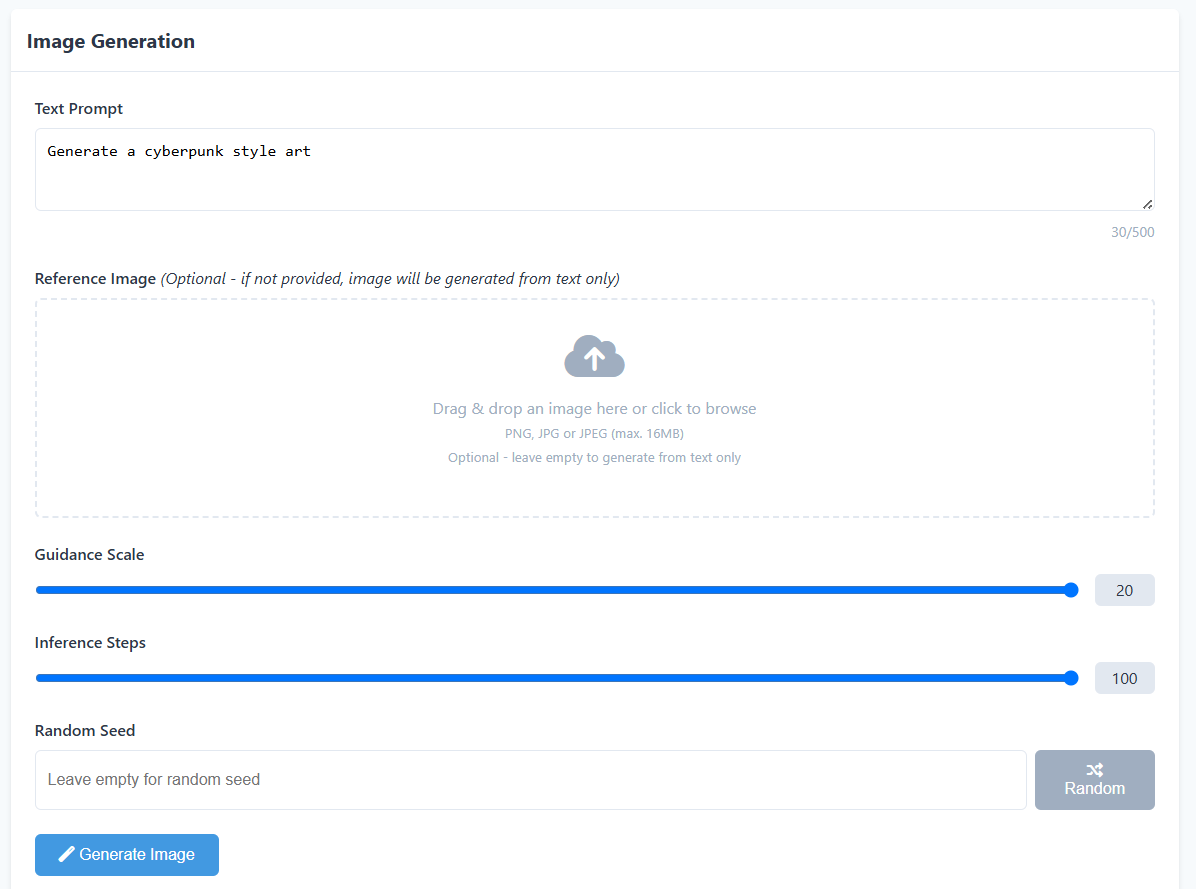
\includegraphics[width=0.75\textwidth]{images/Screenshot 2025-05-02 171143.png}
    \caption{Analytics workbench: K-Means clustering output with Recharts visualisation.}
    \label{fig:analytics-cluster}
\end{figure}

\begin{figure}[h!]
    \centering
    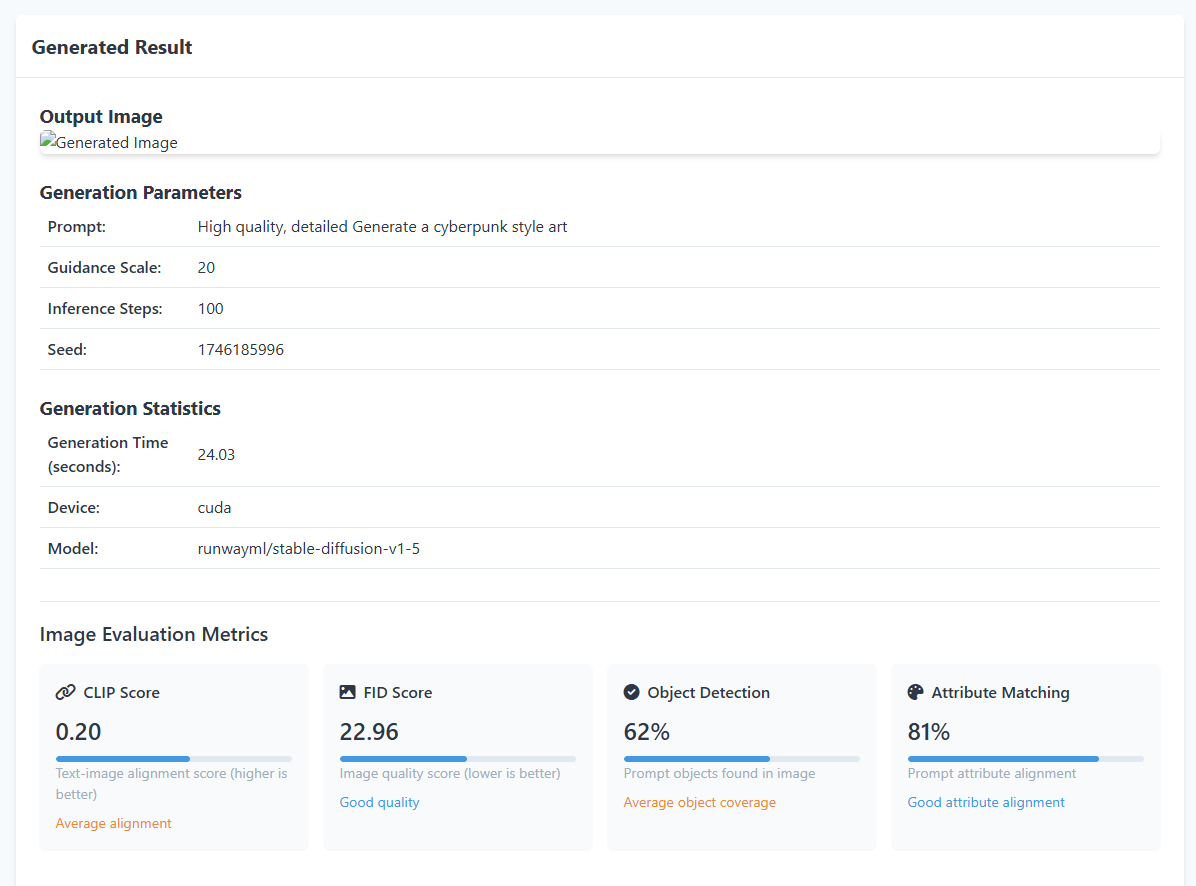
\includegraphics[width=0.75\textwidth]{images/Screenshot 2025-05-02 171207.png}
    \caption{Analytics AI insight generation: correlation and outlier summary from uploaded CSV.}
    \label{fig:analytics-insight}
\end{figure}

\begin{figure}[h!]
    \centering
    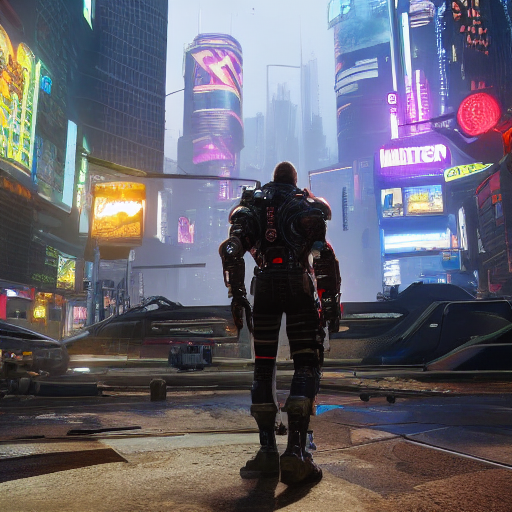
\includegraphics[width=0.75\textwidth]{images/output_1744276115_707c1e28.png}
    \caption{Load test visualisation: request rate and P95 latency over the 5-minute ramp cycle.}
    \label{fig:loadtest}
\end{figure}

\begin{figure}[h!]
    \centering
    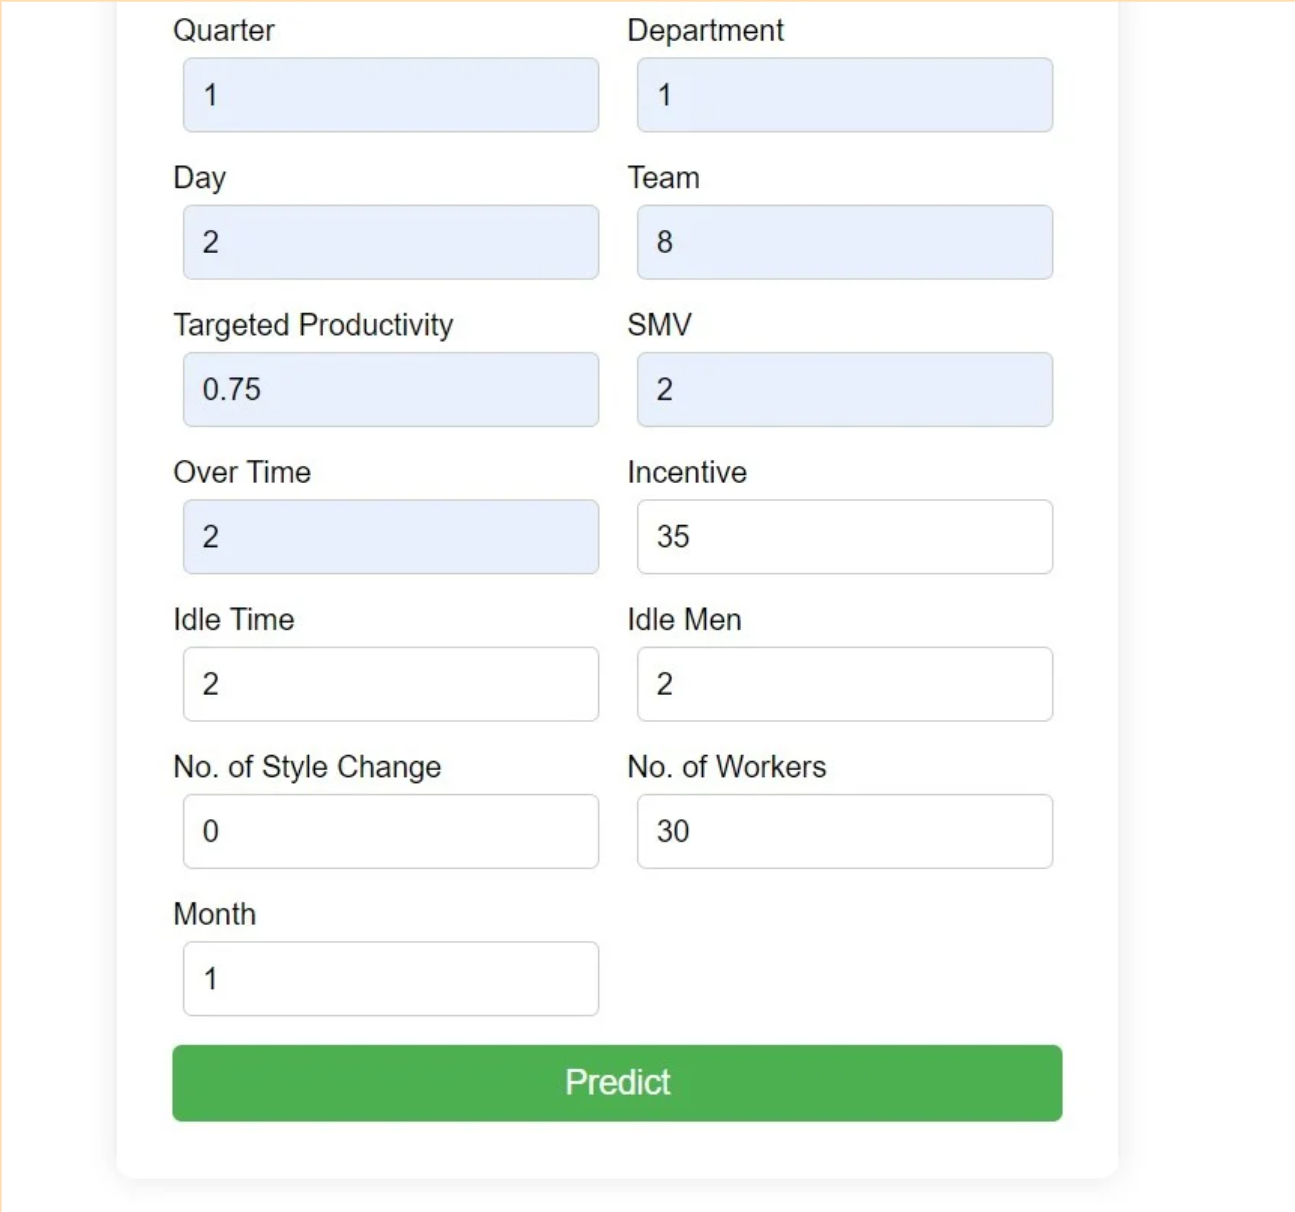
\includegraphics[width=0.75\textwidth]{images/values.png}
    \caption{Quality metric distribution across 3,421 logged interactions (structure, density, naturalness, confidence).}
    \label{fig:quality-dist}
\end{figure}
